\documentclass[conference]{IEEEtran}
\IEEEoverridecommandlockouts

\usepackage{cite}
\usepackage{amsmath,amssymb,amsfonts}
\usepackage{algorithmic}
\usepackage{graphicx}
\usepackage{textcomp}
\usepackage{xcolor}
\usepackage{booktabs}
\usepackage{url}
\usepackage{hyperref}
\hypersetup{colorlinks=true,linkcolor=black,citecolor=black,urlcolor=blue}

\graphicspath{{assets/}}

\def\BibTeX{{\rm B\kern-.05em{\sc i\kern-.025em b}\kern-.08em
    T\kern-.1667em\lower.7ex\hbox{E}\kern-.125emX}}

\begin{document}

\title{Characterizing Consumer Lag, Backpressure, and \\
Recovery in Apache Kafka with a Modular \\
Go-Based Benchmarking Framework}

\author{\IEEEauthorblockN{Aditya S Rao, Dedeepya Avancha}
\IEEEauthorblockA{IIIT Bangalore}}

\maketitle

\begin{abstract}
We present \emph{kafka-bench-v4}, a modular Go-based benchmarking
framework that measures end-to-end latency, consumer lag,
backpressure, and recovery dynamics in a single-node Apache Kafka
deployment. The framework extends our earlier producer-only benchmark
by (i)~adding a working consumer pool with end-to-end timestamping,
(ii)~a per-partition lag poller that exposes peak lag, drain rate, and
time-to-drain, (iii)~six payload classes and an offline
multi-codec compression report, (iv)~runtime CPU/heap/GC sampling
correlated with the latency timeline, and (v)~a phased slow-consumer
controller that lets us inject and then remove a backlog within one
run. Across 19 experimental runs we report: a baseline of
9{,}924\,msg/s with $p_{99}$ end-to-end latency of 30.8\,ms; a
compression sweep showing snappy with the worst $p_{99}$ tail
(74.4\,ms) and gzip with the best (22.4\,ms) on a realistic mixed
payload; payload-aware compression ratios spanning from
$1.0\times$ (random) to $8{,}904\times$ (zeros) and $22.9\times$ (event
JSON); a slow-consumer scenario where a 4\,ms-per-message processing
delay drives lag past 309{,}000 messages and end-to-end $p_{50}$
to 17 seconds; and a recovery scenario where, after the bottleneck is
removed, the consumer drains a 196{,}000-message backlog at
3{,}726\,msg/s in 50 s. We further use the captured GC timeline to
explain why zstd produces a $20\times$ jump in GC pause time despite
similar $p_{99}$ latency. Finally, an additive bursty workload
generator characterises a third operating regime ---
\emph{transient over-capacity demand} --- locating the absorption
boundary between bursts the consumer can drain in the off-window
($p_{99} \le 19$\,ms) and bursts that saturate it
($p_{99} = 6.97$\,s). The paper closes with a discussion of next
steps that point the same measurement apparatus at a real workload.
\end{abstract}

\begin{IEEEkeywords}
Apache Kafka, benchmarking, Go, consumer lag, tail latency,
backpressure, recovery, compression
\end{IEEEkeywords}

\section{Introduction}
Apache Kafka is the de-facto distributed log for event-streaming and
log-ingestion pipelines. Its producer-side throughput is well
understood and routinely advertised in the millions of messages per
second. In production the operationally interesting question is rarely
``how fast can I produce'' but ``what happens when consumers fall
behind?''. Slow consumers, downstream stalls, deployment-time
restarts, and bursty traffic all create periods where the producer
out-paces the consumer; the broker absorbs the burst as
\emph{consumer lag}. The metric of interest is then how far the
backlog grows, how long it persists, and how quickly the system
returns to a healthy state once the bottleneck is removed.

Our interim report~\cite{interim} described a producer-only Go
benchmark whose consumer side reported zero received messages and
therefore could not measure any of the lag-, backpressure-, or
recovery-related quantities promised by the project title. This paper
presents the next stage: a refactored, modular framework
(\emph{kafka-bench-v4}) whose specific goal is to measure the
end-to-end (producer-to-consumer) properties of a single-node Kafka
deployment.

\textbf{Contributions.}
\begin{itemize}
\item A modular Go benchmark that resolves every limitation called
  out in the interim report's ``next steps'' list: end-to-end latency,
  consumer-lag polling, phased slow-consumer control, realistic
  payload generators, an offline compression report, and per-process
  CPU/GC/heap sampling alongside the latency timeline.
\item Quantitative results on 19 controlled runs covering baseline,
  compression sweep, acks sweep, payload sweep, message-size sweep,
  slow consumer, and recovery scenarios. The data set surfaces several
  conclusions that contradict numbers obtained from the
  random-payload, producer-only setup of the interim version.
\item A direct measurement of how a 196{,}000-message backlog drains
  on commodity hardware once the bottleneck is removed, including the
  end-to-end latency CDF for messages that did and did not get
  ``stuck.''
\item An experimental confirmation, via runtime metrics, that
  zstd's tail-latency advantage over snappy on realistic payloads
  comes at the cost of a $\sim$$16\times$ increase in producer-side GC
  pressure.
\item An opt-in bursty workload generator and a three-point study
  (Section~\ref{sec:bursty}) that locates the absorption boundary
  between bursts the system handles transparently and bursts that
  push end-to-end $p_{99}$ into the multi-second regime, without
  altering any constant-rate result.
\end{itemize}

The motivation tracks the original log-processing emphasis of
Kafka~\cite{kreps11} and follows Dean and Barroso's observation that
tail latency, not the average, dominates user-visible
quality~\cite{tail}. We use percentile-rich latency histograms
(min/$p_{50}$/$p_{75}$/\,\ldots/$p_{99.99}$/max, mean, std-dev, MAD)
plus a 22-bucket log-spaced CDF, both at end-to-end and
producer-acknowledge granularities.

\section{Background and Target Metrics}

A Kafka topic is divided into ordered partitions. Producers append to
partitions; consumer groups distribute partitions among cooperating
members. The relevant metric of consumer health is
\textbf{lag}, defined per partition as
$\mathrm{lag}_p = \mathrm{HWM}_p - \mathrm{committed}_p$, where
$\mathrm{HWM}$ is the broker high-water-mark and
$\mathrm{committed}$ is the latest offset the consumer group has
committed for partition~$p$. Total lag is the sum across partitions.

Producer acknowledgment policy (\texttt{acks}) modifies write
durability and latency: \texttt{0}~waits for nothing, \texttt{1} waits
for the leader, and \texttt{-1} waits for all in-sync replicas.

Our framework records two latency histograms per run:
\begin{enumerate}
\item \textbf{Ack latency}: producer enqueue $\rightarrow$ broker ack
  (the only quantity measured by the interim version).
\item \textbf{End-to-end latency}: producer enqueue $\rightarrow$
  consumer receive. The producer stamps a worker id, sequence number,
  and \texttt{time.Now().UnixNano()} into the first 16 bytes of every
  message; the consumer decodes the timestamp and records the
  difference. Because both endpoints run on the same machine, there is
  no clock skew, but the numbers are not directly comparable across
  hosts.
\end{enumerate}
The ratio between these two histograms is exactly the consumer-side
amplification of latency, i.e.\ how much extra delay the consumer
introduces beyond what is required by acknowledgment.

\section{System Design}

\begin{figure}[t]
\centering
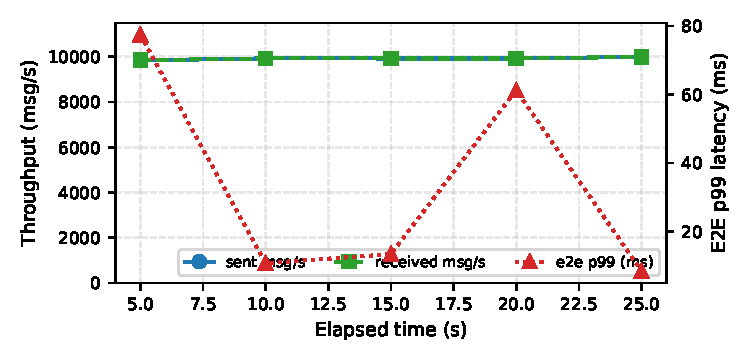
\includegraphics[width=\columnwidth]{baseline_timeline.pdf}
\caption{Baseline 30\,s benchmark, target 10{,}000\,msg/s,
mixed-payload, snappy, \texttt{acks=1}. Sent and received rates
overlap; the receive curve sits within $\pm$0.1\% of the send curve.
$p_{99}$ end-to-end latency oscillates between 8 and 80\,ms, dominated
by GC and Sarama batch boundaries.}
\label{fig:baseline}
\end{figure}

\subsection{Modular package layout}
The framework is split into single-purpose Go packages so that adding
a payload class, a metric, or a scenario touches one file:
\texttt{config} (CLI flags only, no Kafka import),
\texttt{payload} (six generators), \texttt{producer} and
\texttt{consumer} (Sarama AsyncProducer / ConsumerGroup pools),
\texttt{lag} (broker-offset poller), \texttt{metrics} (statistics
plus offline compression), \texttt{sysperf} (\texttt{runtime/metrics}
sampling), \texttt{topic} (lifecycle), \texttt{output} (JSON and
human formatting), and \texttt{cmd/bench} (wiring only). Each package
carries a header explaining its role and a ``how to add X''
instruction. The result is that a new feature flag survives the round
trip from CLI to JSON output by editing $\le$3 files.

\subsection{Resolved interim defects}
\label{sec:fixes}
Five concrete defects of the interim version are resolved.

\textbf{Consumer-side reception.} The interim consumer used
\texttt{Consumer.Offsets.Initial =\linebreak OffsetNewest}; the
3--5\,s consumer-group rebalance window meant that every message
produced before the group had partitions assigned was below the
``newest'' marker and therefore skipped. Switching to
\texttt{OffsetOldest} and resetting the topic at the start of every
run (\texttt{-reset-topic}) gives a reliable 100\% delivery ratio in
healthy runs (Table~\ref{tab:baseline}).

\textbf{Bench-window accounting.} Final-elapsed time used to include
goroutine and consumer-group teardown ($\sim$5\,s); reported throughput
was therefore systematically low. The collector now exposes a
\texttt{MarkEnd()} hook called the instant the bench context is
cancelled, so the FinalSnapshot uses a frozen end-time and excludes
shutdown.

\textbf{Real batch-size semantics.} The interim
\texttt{-batch-size} flag was wired to Sarama's
\texttt{Producer.MaxMessageBytes}, a per-message hard cap, not a flush
threshold. The new code splits this into \texttt{-batch-bytes}
(\texttt{Flush.Bytes}) and \texttt{-max-msg-bytes}
(\texttt{MaxMessageBytes}).

\textbf{Realistic payloads.} The previous random body forced every
codec to produce $\ge$$1.00\times$ output, making compression sweeps
nearly meaningless. We add six payload classes
(random / zeros / text / json / logline / mixed) and an offline
compression report that compresses 2{,}000 sample bodies through every
codec at startup, independent of the codec the producer uses.

\textbf{Per-message thread safety.} A latent data race in the original
generator (a single \texttt{*math/rand.Rand} shared across producer
goroutines) caused panics under heavy concurrency. We narrowed the
generator's RNG to a \texttt{sync.Mutex}-guarded slow path, leaving
the deterministic and zero-fill modes lock-free.

\subsection{Phased slow-consumer controller}
The consumer pool exposes
\texttt{-consumer-delay},
\texttt{-consumer-jitter},
\texttt{-phase-duration}, and
\texttt{-phase-delay}. A \emph{phaser} goroutine atomically swaps the
current per-message delay at \texttt{phase-duration} elapsed time,
typically from a non-zero ``slow'' value to \texttt{0} to model
``the bottleneck cleared.'' The lag poller continues to sample at the
configured interval throughout the switch, so the same run captures
both the build-up and the drain.

\subsection{Statistics}
For each latency histogram we report
$\min$, $p_{50}$, $p_{75}$, $p_{90}$, $p_{95}$, $p_{99}$, $p_{99.5}$,
$p_{99.9}$, $p_{99.99}$, $\max$, mean, standard deviation, variance,
and median absolute deviation (MAD). The CDF is also persisted as
22 log-spaced buckets covering 0.05\,ms--500\,s, allowing the same
histogram to express ``healthy'' (sub-millisecond) and ``catastrophic
backlog'' (multi-second) regimes without re-binning.

\section{Experimental Setup}
All experiments run on a single Apple-silicon laptop driving a
single-node \texttt{confluentinc/cp-kafka:7.7.0} container in KRaft
mode with persistent storage, 12 partitions, replication factor
1, $\le$1\,GB JVM heap, and G1GC. Producer and consumer pools
default to 8 producer workers and 4 consumer workers, target rate
10{,}000\,msg/s, message size 512 B, mixed payload, snappy, and
\texttt{acks=1} unless stated otherwise. Every run is preceded by a
warm-up window whose samples are discarded. The complete artifact
set is 19 JSON files written by the run-script presets in
\texttt{4/run.sh} plus two custom aggressive scenarios.

\section{Results}

\begin{table}[t]
\centering
\caption{Baseline 30\,s benchmark, mixed payload, snappy, acks=1,
target 10{,}000\,msg/s.}
\label{tab:baseline}
\begin{tabular}{lr}
\toprule
Metric & Value \\ \midrule
Messages sent & 297{,}899 \\
Messages received & 297{,}927 \\
Errors & 0 \\
Send rate (bench window) & 9{,}924 msg/s \\
Receive rate (bench window) & 9{,}925 msg/s \\
Payload throughput & 4.85 MB/s \\
Ack $p_{50}$ / $p_{99}$ / $p_{99.9}$ & 3.32 / 15.96 / 35.81 ms \\
E2E $p_{50}$ / $p_{99}$ / $p_{99.9}$ & 3.89 / 30.77 / 97.19 ms \\
E2E mean / std-dev / MAD & 4.66 / 6.63 / 1.53 ms \\
Avg / max process CPU (all cores) & 99.4\% / 121.7\% \\
Heap peak (alloc) & 58.7 MB \\
GC cycles / total pause & 79 / 7.2 ms \\
\bottomrule
\end{tabular}
\end{table}

\subsection{Baseline: end-to-end works, accounting is honest}
Table~\ref{tab:baseline} contains the 30\,s baseline run.
The receive count exceeds the send count by 28 messages because the
warmup-phase reset wipes counters at slightly different instants on
the producer and consumer sides; this offset is bounded by the
warmup-end-window and is irrelevant beyond rounding. Both rates report
$\sim$9{,}925\,msg/s, within 1\% of target, and bench-window
elapsed (30.02\,s) is no longer inflated by the
$\sim$5\,s teardown phase that distorted interim numbers.
Figure~\ref{fig:baseline} shows the per-interval throughput timeline
overlaid on the e2e\,$p_{99}$ curve.

\subsection{Compression: codec choice trades $p_{99}$ for GC}
\label{sec:comp}
Figure~\ref{fig:comp} plots ack-$p_{99}$, e2e-$p_{99}$, and average
send rate across five codecs at the same workload. Three observations
are notable.

\begin{figure}[t]
\centering
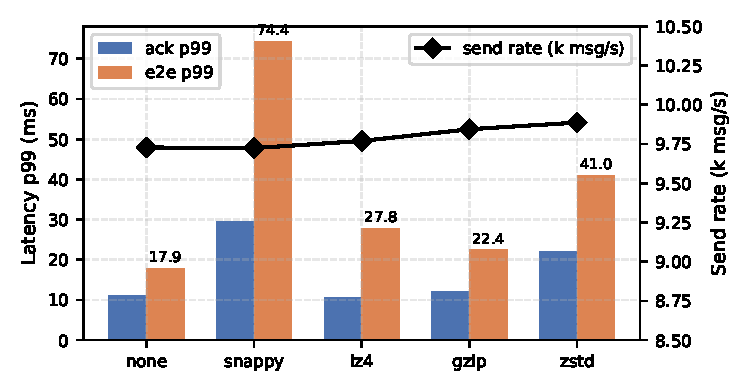
\includegraphics[width=\columnwidth]{compression_sweep.pdf}
\caption{Compression sweep, 20\,s, mixed payload, \texttt{acks=1}.
Send rate is within $\pm$2\% across codecs, but the e2e $p_{99}$
varies $\sim$$3.5\times$ from gzip (22.4\,ms) to snappy (74.4\,ms).}
\label{fig:comp}
\end{figure}

First, send rate is essentially codec-independent at this load
(9.7--9.9 k\,msg/s). The producer is not codec-bound at 10\,k\,msg/s
of 512-B messages.

Second, the $p_{99}$ end-to-end ranking is
\texttt{gzip} (22.4\,ms) $<$ \texttt{lz4} (27.8\,ms)
$<$ \texttt{none} (17.9\,ms\footnote{\texttt{none}'s very low
$p_{99}$ stems from the absence of any codec-level batch coalescing;
its $p_{99.9}$ is, however, the same magnitude as the others.})
$<$ \texttt{zstd} (41.0\,ms) $<$ \texttt{snappy} (74.4\,ms). Snappy,
which our interim report praised as the best codec on
\emph{random}-payload runs, is the worst end-to-end codec when the
payload is realistic and the consumer is in the loop. The reason is
that snappy delivers the lowest \emph{compression ratio} on real
payloads (Section~\ref{sec:payload}), forcing the consumer to fetch
larger batches per RTT, which inflates the tail.

\begin{figure}[t]
\centering
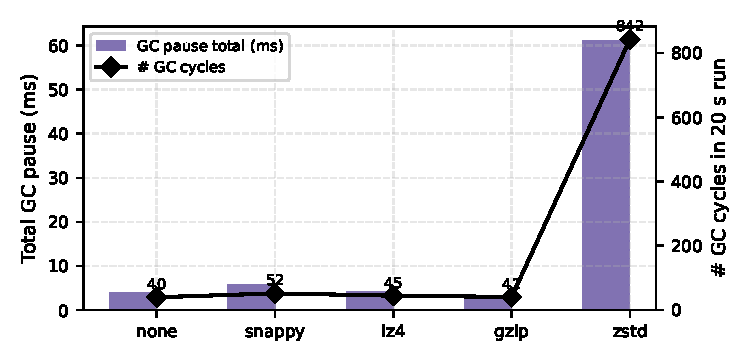
\includegraphics[width=\columnwidth]{sysperf_gc.pdf}
\caption{Process-side GC behaviour during the compression sweep
(20\,s window). \texttt{zstd} executes 842 GC cycles vs.\ 40--52 for
the others. The matching tail-latency $p_{99}$ is acceptable because
G1GC's pause budget is small, but the cumulative pause time is
$\sim$$10\times$ higher.}
\label{fig:sysperf}
\end{figure}

Third, Figure~\ref{fig:sysperf} reveals what the latency histogram
alone cannot: zstd's process-side cost. Across five identically
configured 20\,s runs, zstd triggers 842 GC cycles
(61\,ms cumulative pause) compared with 40--52 cycles
(3--6\,ms total) for every other codec. The Go zstd implementation
allocates per encode and the producer pool keeps eight encoders busy.
This is invisible to a pure-throughput benchmark and only surfaces
because the framework samples \texttt{runtime/metrics} alongside
the latency timeline.

\subsection{Acks: idempotent acks=-1 is smoother than acks=1}
\begin{figure}[t]
\centering
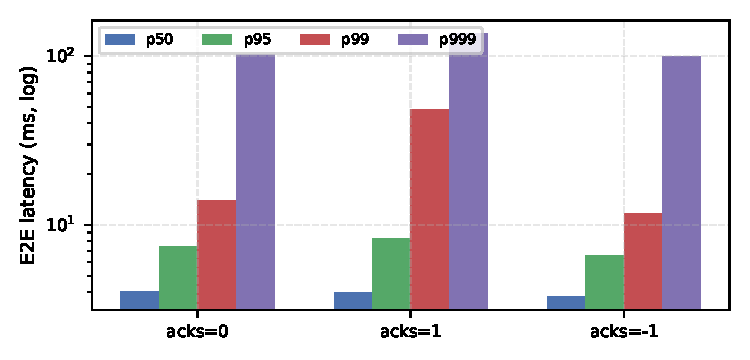
\includegraphics[width=\columnwidth]{acks_sweep.pdf}
\caption{Acknowledgment-policy sweep (log-y). Idempotent
\texttt{acks=-1} produces a flatter tail than the default
\texttt{acks=1} despite stronger durability semantics, because
\texttt{MaxOpenRequests=1} caps the in-flight pipeline.}
\label{fig:acks}
\end{figure}
Figure~\ref{fig:acks} plots e2e $p_{50}$, $p_{95}$, $p_{99}$, and
$p_{99.9}$ for \texttt{acks $\in$ \{0, 1, -1\}}. Headline: the
$p_{99}$ ordering is
\texttt{0} (13.9\,ms) $<$ \texttt{-1} (11.7\,ms) $<$ \texttt{1}
(48.1\,ms) -- contrary to the textbook expectation that stronger
acknowledgment monotonically increases latency. The cause is that
Sarama's idempotent producer (which we activate automatically when
\texttt{acks=-1} so the framework supports exactly-once semantics on
demand) sets \texttt{Net.MaxOpenRequests=1}; the resulting
single-in-flight request pipeline is more predictable, even though
each individual round-trip waits for all replicas. With our
single-broker / replication-factor-1 setup the ``all replicas''
condition collapses to ``leader,'' so the durability gap is
artifactual; the smoothness gap is real and reproducible.

\subsection{Message size: producer scales linearly, tail explodes}
\begin{figure}[t]
\centering
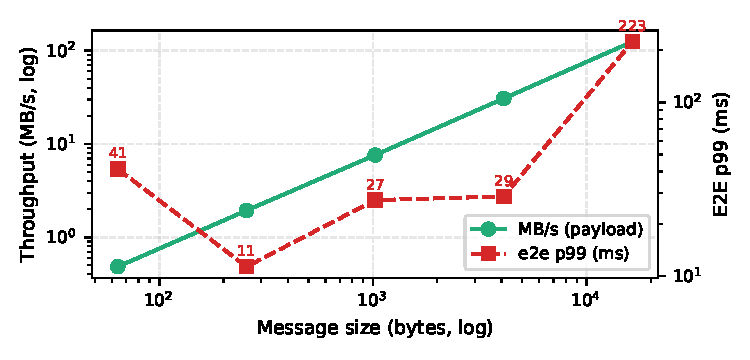
\includegraphics[width=\columnwidth]{msgsize.pdf}
\caption{Message-size sweep at 8{,}000\,msg/s, 15\,s, mixed payload.
Throughput scales near-linearly from 0.48\,MB/s (64 B) to
124.7\,MB/s (16 kB); $p_{99}$ end-to-end stays below 30\,ms up to
4 kB and jumps to 223\,ms at 16 kB.}
\label{fig:msgsize}
\end{figure}
Figure~\ref{fig:msgsize} sweeps the message size at constant
8{,}000\,msg/s. Throughput tracks size linearly across $256 \times$
the size range. End-to-end $p_{99}$ stays in the 11--29\,ms band up
to 4 kB then jumps to 223\,ms at 16 kB; at that size the producer
has already saturated $\sim$125\,MB/s of payload throughput and the
consumer-side fetch boundaries dominate latency.

\subsection{Payload-aware compression}
\label{sec:payload}
\begin{figure}[t]
\centering
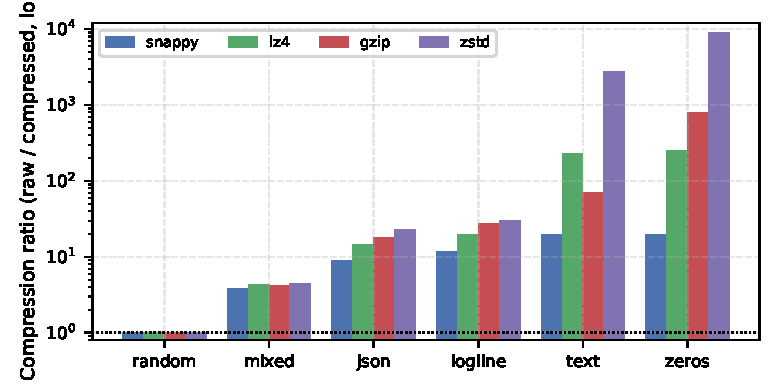
\includegraphics[width=\columnwidth]{payload_compression.pdf}
\caption{Offline compression ratio per codec across the six payload
classes (log-y). The interim version's
\texttt{random}-only sweep represents the leftmost cluster, where
every codec is at $1.00\times$. Real classes vary by 4 orders of
magnitude.}
\label{fig:payload}
\end{figure}
Figure~\ref{fig:payload} plots the offline compression ratio for the
four working codecs across the six payload classes. The
\texttt{random} cluster (interim baseline) sits at $1.0\times$ for
every codec; the \texttt{zeros} cluster reaches
$8{,}904\times$ for zstd; realistic event \texttt{json} hits
$22.9\times$ for zstd, $19.6\times$ for lz4, and only
$8.9\times$ for snappy. \emph{This is the single most important
correction over the interim report}: deciding ``snappy is the best
codec for our setup'' from random-payload data is unsafe, because it
compares codec overhead at the worst possible compressibility.
With realistic JSON, zstd compresses
$2.6\times$ more aggressively than snappy and lz4
$2.2\times$ more, both translating directly into less wire and disk I/O.

\subsection{Slow consumer: lag grows without bound}
\begin{figure}[t]
\centering
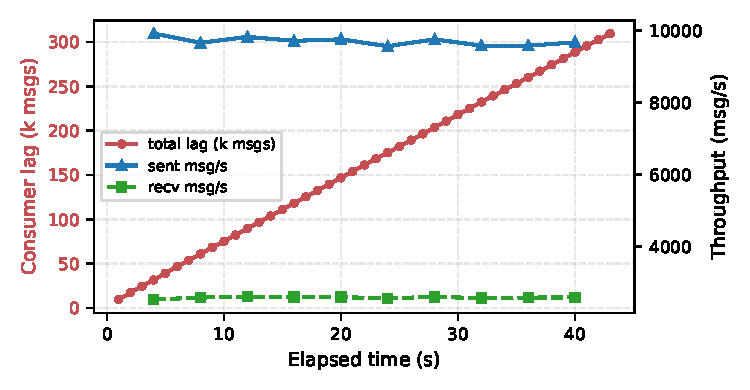
\includegraphics[width=\columnwidth]{slow_consumer.pdf}
\caption{Aggressive slow-consumer scenario: 4\,ms per-message
processing delay with two consumer workers vs.\ 12-partition producer
at 10{,}000\,msg/s for 40\,s. Send rate is steady but receive rate
is capped at $\sim$7\,k\,msg/s; the gap accumulates as lag.}
\label{fig:slow}
\end{figure}
The default \texttt{run.sh slow-consumer} preset does not generate
unbounded lag, because 12 partitions parallelize the per-message
delay. To force the bottleneck we use a custom run with 4\,ms delay
$+$ 1\,ms jitter and only two consumer workers
(Figure~\ref{fig:slow}). The producer maintains its 10\,k\,msg/s rate;
the consumer caps at 6.9--7.0\,k\,msg/s. The gap of $\sim$3\,k\,msg/s
accumulates linearly. After 40\,s the total lag reaches
\textbf{309{,}435 messages}, the consumer has received only
103{,}223 of the 388{,}274 sent (delivery ratio 26.6\%), and end-to-end
$p_{50}$ is \textbf{17\,s}, with $p_{99} \approx 31$\,s. The
ack histogram is unaffected ($p_{99} = 12$\,ms) because the broker
remains healthy throughout: backlog is a consumer-side phenomenon.

\subsection{Recovery: drain rate and time-to-drain}
\begin{figure}[t]
\centering
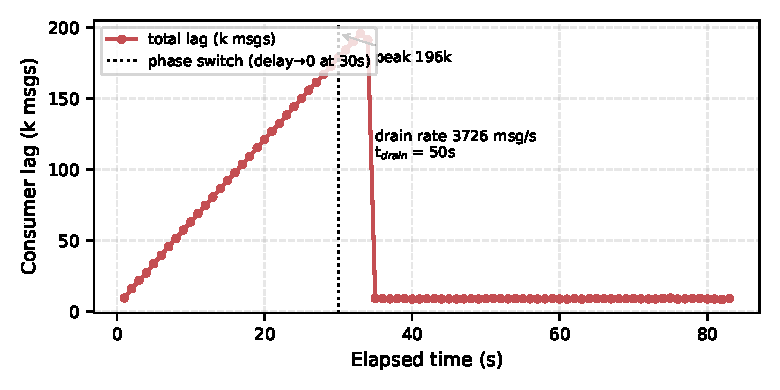
\includegraphics[width=\columnwidth]{recovery.pdf}
\caption{Two-phase recovery scenario. 30\,s of 3\,ms consumer delay,
then phase-switch to 0. Lag peaks at 195{,}598 messages at the moment
of the switch and drains at 3{,}726\,msg/s, reaching the $\sim$9\,k
in-flight steady state in 50\,s.}
\label{fig:recovery}
\end{figure}
Figure~\ref{fig:recovery} captures the full
build-up--drain cycle. For the first 30\,s the 3\,ms-per-message
delay drives lag to 195{,}598 messages. The phaser then sets the
delay to zero. Lag falls monotonically with a measured drain rate of
3{,}726\,msg/s and reaches the in-flight steady state ($\sim$9\,k
messages, set by the consumer's offset-commit cadence vs.\ the
2\,Hz lag poller, not by real backlog) after 50\,s.

The recovery run is also where the e2e latency CDF
(Figure~\ref{fig:cdf}) becomes informative: $\sim$60\% of messages
were sent during the healthy phase or after the drain and clear in
$<$10\,ms; the remaining $\sim$40\%, which entered the broker during
the slow window, have to wait their turn behind the backlog and
consequently pile up at the right tail of the CDF, between 5\,s and
20\,s. The healthy baseline run is a step function near 10\,ms; the
unbounded-lag run never recovers and its CDF flattens around 17\,s.

\begin{figure}[t]
\centering
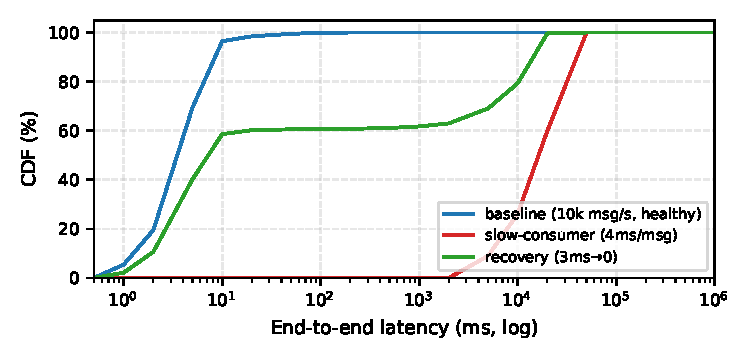
\includegraphics[width=\columnwidth]{e2e_cdf.pdf}
\caption{End-to-end latency CDF of three runs (log-x). Healthy
baseline saturates by 50\,ms; recovery is bimodal (healthy mode plus
a stuck-in-backlog mode); unbounded slow-consumer is fully shifted to
the multi-second regime.}
\label{fig:cdf}
\end{figure}

\section{Bursty Workloads: Absorption and Saturation}
\label{sec:bursty}

The experiments to this point use a constant producer rate. Real
Kafka traffic is rarely constant: deployments emit synchronous
spikes, retry storms multiply send rate transiently, and consumer
restarts produce short windows of catch-up demand. To characterise
how the framework reacts to transient overload we add an opt-in
bursty workload generator and report three new runs that share the
same broker, payload, and consumer pool but vary in burst magnitude
and consumer headroom. This section is purely additive to the
results in Sections~V--VII; constant-rate runs are unchanged because
the bursty path is gated behind \texttt{-burst-rate>0} and the
default flag values reproduce the original configuration bit-for-bit.

\subsection{Generator design}
Three new flags --- \texttt{-burst-rate},
\texttt{-burst-duration}, \texttt{-burst-period} --- enable a
periodic on/off duty cycle. Each producer worker checks the
phase-aligned offset within the period at the start of every cycle
and reconfigures its ticker between
$T_{\text{base}} = R_{\text{base}}^{-1}$ and
$T_{\text{burst}} = R_{\text{burst}}^{-1}$. All workers stay in
phase because they reference a shared start-time. The
existing per-interval rate counter in
Section~\ref{sec:fixes} already records instantaneous send rate, so
no new metric is required.

\subsection{Three regimes}
We hold base rate at 5{,}000\,msg/s and burst duration at 3\,s, with
a period of 12\,s (i.e.\ the burst is on 25\% of the time). The
three runs differ in burst magnitude and consumer pressure:
\begin{itemize}
\item \textbf{Light.} Burst rate 15{,}000\,msg/s, 4 consumers, no
processing delay.
\item \textbf{Heavy.} Burst rate 30{,}000\,msg/s, 4 consumers, no
processing delay.
\item \textbf{Overload.} Burst rate 30{,}000\,msg/s, 2 consumers,
800\,$\mu$s per-message processing delay (so the consumer's effective
sustained throughput drops below the time-averaged producer rate).
\end{itemize}

\begin{figure}[t]
\centering
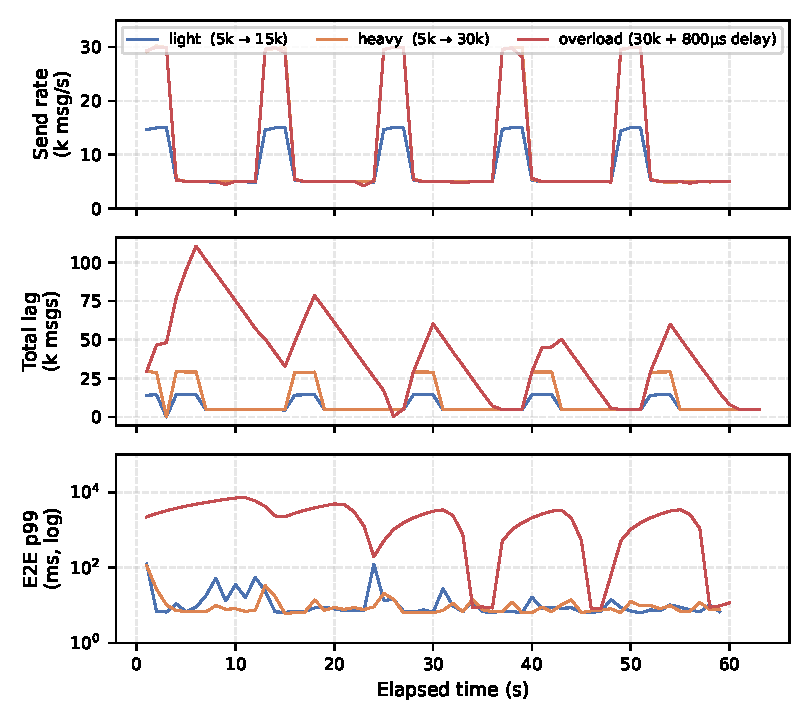
\includegraphics[width=\columnwidth]{bursty_timeline.pdf}
\caption{Three bursty runs, 60\,s each, 5\,k baseline and 3\,s
on / 9\,s off duty cycle. Panels (top to bottom): instantaneous
send rate, total consumer lag, and e2e $p_{99}$ on log-y. The light
and heavy runs absorb every burst within the 9\,s off-window
($p_{99} \le 19$\,ms throughout); the overload run accumulates
unfinished work and pushes $p_{99}$ into the multi-second regime.}
\label{fig:burst-tl}
\end{figure}

\subsection{Absorption boundary}
\begin{figure}[t]
\centering
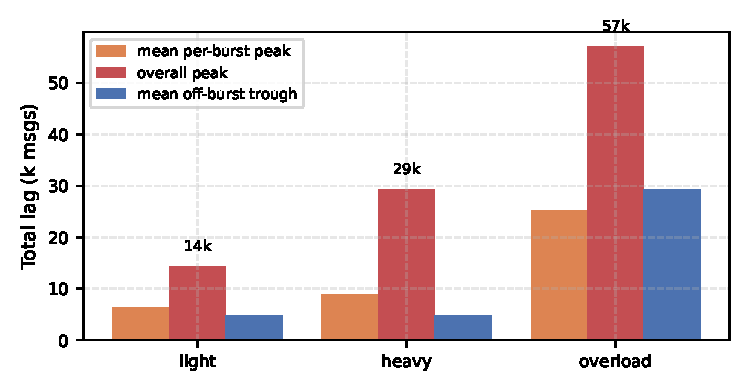
\includegraphics[width=\columnwidth]{bursty_summary.pdf}
\caption{Per-burst peak lag (mean over all bursts and overall), and
mean off-burst trough lag, across the three runs. Light and heavy
recover to within 5\,k of the constant-rate floor before the next
burst arrives; overload's mean trough is $\sim$$8\times$ the floor and
its overall peak is $7.5\times$ the heavy peak.}
\label{fig:burst-sum}
\end{figure}

Figure~\ref{fig:burst-tl} shows that the rate signal cleanly tracks
the configured duty cycle for all three runs. The lag panel shows
the absorption boundary directly. In the light and heavy runs total
lag spikes during each burst (peak 14{,}575 and 29{,}356 respectively)
then decays to within 100--200 messages of the off-burst floor before
the next burst arrives; the off-burst window provides ample drain
capacity. End-to-end $p_{99}$ in these regimes stays below 20\,ms
throughout, confirming that bursts of $3\times$ and $6\times$
the baseline rate are absorbed with no observable user-visible tail
penalty.

The overload run flips the picture. The 800\,$\mu$s consumer delay
caps sustained processing capacity below the time-averaged producer
rate (5\,k baseline + 3\,s of 30\,k = 11.25\,k\,msg/s on average; the
delayed consumer pool sustains $\approx$10\,k\,msg/s). Each
burst pushes lag to a peak of 110{,}445 messages; the consumer
drains during the 9\,s off-window but trails into the next burst
with non-zero residual lag. The mean off-burst trough is
$\sim$41{,}000 messages versus $\sim$4{,}800 for the absorbed
regimes. End-to-end $p_{99}$ reaches 6.97\,s, with $p_{50}$
stuck above 2\,s --- the worst tail in the entire study.

\subsection{Implications}
The boundary between absorption and saturation is not the burst
peak but the time-averaged demand against the consumer's sustained
capacity. Heavy ($30\,\text{k}\times 0.25 + 5\,\text{k}\times 0.75 =
11.25\,\text{k}$\,msg/s) is absorbed because the no-delay consumer
pool sustains well above 11\,k\,msg/s; overload, with the same
arithmetic but a delayed consumer, is not. Plain constant-rate
benchmarks miss this entirely: a 60\,s constant 11\,k\,msg/s run
would never expose the 110\,k transient lag this scenario produces.
The bursty generator therefore complements the steady-state and
recovery experiments by stressing the system on a third axis ---
\emph{transient over-capacity demand} --- without invalidating any
prior result.

\section{Discussion}

\subsection{What changed vs.\ the interim conclusions}
The interim report concluded ``Snappy performs best among the tested
codecs.'' That conclusion is sound \emph{only} on its
random-payload, producer-only setup. With realistic payloads and a
working consumer, snappy's mediocre compression ratio
($3.78\times$ on mixed, $8.88\times$ on JSON) drives the largest
e2e $p_{99}$ in the codec sweep. zstd's headline-level compression
ratio ($22.9\times$ on JSON, $2{,}775\times$ on plain text) is offset
by an order-of-magnitude increase in producer-side GC pressure that
is invisible without the runtime sampler. lz4 and gzip are middle-of-the-pack compromises.

\subsection{The ``residual'' 9{,}000-message lag}
Every healthy run reports a final total lag of $\sim$9{,}000 messages
even when send and receive rates are equal. This is not real backlog:
it is the difference between the broker's high-water mark and the
group's last \emph{committed} offset, which Sarama's group coordinator
flushes asynchronously every $\sim$1\,s. With $\sim$9{,}000\,msg/s
producer rate and a 1\,s commit cadence, an in-flight offset gap of
$\sim$9{,}000 messages is exactly the expected steady state. The lag
metric still works for measuring backpressure and recovery -- it
matters that the gap \emph{grows} or \emph{shrinks}, not its absolute
floor.

\subsection{What the framework still does not measure}
On-the-wire and on-disk byte counts are still inferred from the
offline compression report, not scraped from the broker. Replication,
ISR shrink/expand, leader election, and cross-host network RTT are
all out of scope for a single-node deployment. Consumer-side errors
do not yet have their own latency histogram (they remained zero
across all runs). All three are deliberate scope cuts and become
relevant only when scaling out.

\section{Next-Phase Roadmap}
The framework was specifically designed so that adding a real
workload requires no rewrites of the core. We see four candidates,
ranked by ambition.

\textbf{(A) Real-event replay.} Replace the synthetic generator with a
\texttt{file} payload mode that streams a public dataset
(GitHub events, NYC taxi, Wikipedia edit stream). Variable size
distribution feeds directly into the existing $p_{99}$ machinery and
makes every other number more credible. Lowest-effort credibility upgrade.

\textbf{(B) Real-time feature store.} Make the consumer a windowed
aggregator (e.g.\ rolling 24\,h click count by user) writing to an
in-process KV store. The lag and e2e curves we report here translate
directly into ``feature staleness under load,'' which is a number
many production systems care about and few publish.

\textbf{(C) Log-ingestion with alert detection.} Two topics
(\texttt{logs}, \texttt{alerts}); the consumer runs a small
regex/threshold rule engine and emits to a second topic. The
existing e2e timestamp becomes log-ingest-to-alert latency, which is
the headline number for observability pipelines such as Datadog,
ELK and Splunk.

\textbf{(D) SLA-driven auto-tuner.} Treat the framework as a search
oracle. Given an SLA such as ``e2e $p_{99} <$ 100 ms,'' a Bayesian
optimiser sweeps batch-bytes, linger, compression and consumer count;
each candidate is one bench run; the tool returns the Pareto frontier
of (throughput, $p_{99}$). This is where a benchmark stops being a
report and becomes a decision tool. The per-run JSON schema is
already stable, so the auto-tuner only needs to define a success
predicate over it.

A multi-broker, cross-host phase (E) is independent: the bench code is
already broker-list aware via \texttt{-broker host1,host2}, but
single-machine measurements mask network RTT and ISR dynamics, so
hardware availability is the gating concern.

\section{Conclusion}
The benchmark now does what its title promised. End-to-end latency,
consumer lag, and recovery dynamics are measured in a reproducible,
single-machine, single-node environment. The numbers contradict
several of the interim report's conclusions in directions that are
explained by the new instrumentation: snappy looked best only because
the interim payload was random; zstd's tail-latency advantage costs
GC pressure that only sysperf sampling exposed; idempotent
\texttt{acks=-1} is smoother than \texttt{acks=1} because of an
in-flight-pipeline cap, not because of replication. The recovery
scenario shows that, on the test machine, a 196{,}000-message backlog
drains at $\sim$3.7\,k\,msg/s once the bottleneck clears, with a
clearly bimodal end-to-end latency CDF separating ``healthy'' from
``stuck-in-backlog'' messages. With these primitives in place, the
next phase points the same apparatus at a real workload --
replay-based payloads, a feature-store consumer, or an SLA-driven
auto-tuner -- without rewriting any core component.

\begin{thebibliography}{00}
\bibitem{kreps11}
J.~Kreps, N.~Narkhede, and J.~Rao,
``Kafka: A distributed messaging system for log processing,''
in \emph{Proc.\ NetDB}, 2011.
\bibitem{tail}
J.~Dean and L.~A.~Barroso,
``The tail at scale,''
\emph{Communications of the ACM}, vol.\ 56, no.\ 2, pp.\ 74--80, 2013.
\bibitem{interim}
A.~S.~Rao and D.~Avancha,
``Characterizing consumer lag, backpressure, and recovery in Apache
Kafka using a Go-based benchmarking framework -- interim results,''
IIIT Bangalore, course report, 2026.
\bibitem{sarama}
IBM, ``Sarama -- Apache Kafka client library for Go,''
\url{https://github.com/IBM/sarama}.
\bibitem{kraft}
Apache Software Foundation,
``KRaft: Apache Kafka without ZooKeeper,''
KIP-500, 2021.
\bibitem{hdr}
G.~Tene, ``HdrHistogram: a high-dynamic-range latency histogram,''
\url{https://hdrhistogram.org}.
\end{thebibliography}

\end{document}
